\documentclass[a4paper]{article}
\usepackage[margin=1in]{geometry} % full-width
\usepackage[utf8]{inputenc}
\usepackage{hyperref}
\usepackage{graphicx, color}

\title{Online Bookstore JSON API}
\author{Bradley Marques}

\begin{document}
\maketitle

\section{Introduction}

A proof-of-concept bookstore JSON API was developed using Ruby on Rails in a
docker container.
The API allows a user to authenticate by getting a JSON Web Token (JWT).
The API also allows a user to index, show, update, create, and delete books.
Best practice of Test-Driven-Development (TDD) was followed, as well as the
Ruby on Rails ``convention over configuration'' paradigm.
The problem was decomposed into constituent models of a User and a Book
(Section~\ref{sec:domain}).
These two models are expanded upon by considering their database representation
in a relational database (Section~\ref{sec:database}).
The required API endpoints and responses are designed (Section~\ref{sec:api}),
and assumptions about the domain are highlighted (Section~\ref{sec:assumptions}).
Ruby on Rails was chosen because of familiarity and therefore speed of
development, as well as relevant software packages to handle testing, data
seeding, JSON API serialization, etc. (Section~\ref{sec:technology}).
Not all work was completed within the deadline (Section~\ref{sec:work_completed}).
Technical trade-offs are briefly discussed (Section~\ref{sec:trade_offs}) as
well as work required for production readiness (Section~\ref{sec:production}).

\section{Problem Analysis}

\subsection{Domain}
\label{sec:domain}

The domain contains the following models:

\begin{itemize}
  \item \textbf{User} - (a.k.a. Author) the user of the system. Has API
  credentials in the form of username and password and has zero to many books.
  \item \textbf{Book} - a Book that an Author has written and wishes to
  self-publish.
\end{itemize}

\subsection{Models and Database design}
\label{sec:database}

The entity relation diagram below was created before implementation:

\begin{figure}[h]
  \begin{center}
    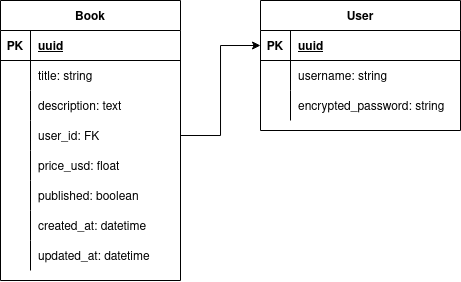
\includegraphics[width=9cm]{images/melio_database_design.png}
  \end{center}
\end{figure}

Some notes:

\begin{itemize}
  \item To prevent ``database walking'' and therefore increase application security,
  universally unique identifiers (uuids) are used instead of sequential database
  ids.
  \item The \texttt{published} and \texttt{encrypted\_password} fields were
  planned but not completed within the four-hour deadline (see
  Section~\ref{sec:work_completed})
\end{itemize}

\subsection{API Endpoints}
\label{sec:api}

The application requires REST endpoints to perform CRUD actions on Book resources.
It is also prudent to version APIs to allow for maintainability when new versions
are developed.

Therefore, the following API endpoints were implemented:

\begin{enumerate}
  \item \texttt{GET base\_url/api/v1/books} to index/list all Books.
  \item \texttt{GET base\_url/api/v1/book/:id} to show a single Book.
  \item \texttt{POST base\_url/api/v1/books} to create a new Book.
  \item \texttt{PATCH base\_url/api/v1/book/:id} to update a Book.
\end{enumerate}

The following API endpoints were planned but not completed within the deadline:

\begin{enumerate}
  \item \texttt{POST base\_url/api/v1/token} to get a new JWT.
  \item \texttt{DELETE base\_url/api/v1/books/:id} to delete/un-publish a Book.
\end{enumerate}

\subsection{Assumptions Made}
\label{sec:assumptions}

The following assumptions are made for the purposes of the proof-of-concept:

\begin{itemize}
  \item This application will be deployed once per bookstore, and there is
  therefore no need to model a ``Store'' in the domain.
  \item There is a one-to-many relationship between a User and Books (i.e. Books
  cannot have multiple Authors, and a User can have zero to many Books).
  \item Book prices are in United States Dollars (USD).
  \item There are no requirements at the moment for user management.
  \item Pagination is not required on the Book list endpoint (i.e. small number
  of resources).
  \item When listing/indexing books, they should be sorted by title in
  alphanumeric order.
\end{itemize}

\section{Choice of Technology}
\label{sec:technology}

The list below summarizes the choice of technology used and gives a brief
justification for each choice:

\begin{itemize}
  \item \textbf{Containerization}: Docker
  \item \textbf{Programming Language}: Ruby 3.1.0 - the latest stable version at time of writing.
  \item \textbf{Framework}: \href{https://rubyonrails.org/}{Ruby on Rails 7.0.1}: chosen for familiarity and therefore speed of development. Latest stable version at time of writing.
  \item \textbf{API standard/specification}: \href{https://jsonapi.org/}{JSON API}: gold-standard for JSON API responses.
  \item \textbf{Database}: \href{https://www.postgresql.org/}{PostgreSQL}: powerful and feature-rich open-source relational database
\end{itemize}

Additionally, the following Rails-specific gems were used:

\begin{itemize}
  \item \textbf{Authentication}: \href{https://github.com/jwt/ruby-jwt}{JWT} as specified by brief.
  \item \textbf{Authorization}: \href{https://github.com/varvet/pundit}{Pundit} - gem for simple OOP authorization.
  \item \textbf{Testing}: \href{https://github.com/blowmage/minitest-rails}{Minitest}
  \item \textbf{Database Seeding}: \href{https://github.com/thoughtbot/factory_bot}{Factory Bot}
  \item \textbf{Seed data generation}: \href{https://github.com/faker-ruby/faker}{Faker}
\end{itemize}

\section{Work Completed and Not Completed Within Deadline}
\label{sec:work_completed}

A four-hour deadline was imposed on the proof of concept, and the entire brief
was not fulfilled. Work successfully completed includes:

\begin{itemize}
  \item Containerization using Docker.
  \item Authentication using JWT (mocked in tests).
  \item Authorization:
  \begin{itemize}
    \item A Book can only be updated by its Author.
    \item A Book can only be deleted by its Author.
  \end{itemize}
  \item JSON REST API to:
  \begin{itemize}
    \item Index all Books as an unauthenticated or authenticated User.
    \item Show a Book as an unauthenticated or authenticated User.
    \item Create a Book as an authenticated User only.
    \item Update a Book as an authenticated User only.
  \end{itemize}
  \item Model tests.
  \item Controller tests.
\end{itemize}

Work not completed in the timeframe includes:

\begin{itemize}
  \item API endpoints to authenticate using JWT (as mentioned, this was mocked
  in tests).
  \item Books have cover images.
  \item Books are searchable by title, author, or description.
  \item Pagination of Book resources on the index endpoint.
\end{itemize}

\section{Technical Trade-offs}
\label{sec:trade_offs}

The following trade-offs were made:

\begin{itemize}
  \item \textbf{Monolithic Application} - as it stands, the application is a
  monolith and is not decomposed into microservices.
  \item \textbf{Multi-author books} - books cannot currently be co-authored.
  \item \textbf{User roles} - at the moment, a User is by default an Author. However, as
  the system grew, it would be prudent to add the idea of a ``role'' such that
  users could be admins to manage the system, bookstore owners to manage stock,
  etc.
  \item \textbf{Pagination} - currently there is no pagination on the books
  index action. If there were millions of books, this endpoint would be unusable.
  \item \textbf{Search} - currently, a user is unable to search through books.
  \item \textbf{Cover Images} - this was deemed out-of-scope. Cover images would
  not sit in the relational database, but would rather sit on something like
  Amazon S3. This is therefore almost a separate system.
\end{itemize}

\section{Work Required for Production Readiness}
\label{sec:production}

To achieve production-readiness, the following is required:

\begin{enumerate}
  \item Complete the brief by completing work currently unfinished (Section~\ref{sec:work_completed})
  \item Decide on hosting for the web application (example: Heroku)
  \item Decide on hosting for the database (example: Heroku PostgreSQL)
  \item Decide on hosting for cover images (example: Amazon S3)
  \item Develop continuous integration and continuous development (CI \& CD) pipeline (example: GitHub actions)
  \item Implement logging (example: \href{https://www.papertrail.com/}{Papertrail})
  \item Implement API documentation for developers to consume
  \item Implement load-balancing if not already provided
  \item Implement API throttling to prevent DDOS attacks
\end{enumerate}

\end{document}
